% !TEX root = ../Report.tex

\subsection{Setup}

The project was created in Python 3.6, NiBabel was used to convert and import the CT scans and the two architectures were built and trained on Tensorflow's high-level API Keras. Furthermore the tool Slicer was used to display the CT scans and to create the 3D model of the lung and bronchus.

\subsection{Training processes}
The training of both networks was done on a Nvidia GTX1080Ti GPU and consumed a large amount of computational resources and RAM storage. Especially the big demand for RAM can be attributed to the fact that we imported the whole dataset at once instead of importing and feeding it to the training process in real time with the above described generator. The training for both networks on the 10 CT scans over 35 epochs took several hours.\newline 
The loss function during training of the DeepMedic architecture is shown in figure \ref{train_deepmedic}. The BCE loss for the lungs converges very fast to an asymptote close to 0. The loss for the bronchus is less stable and decreases slower. It furthermore remains higher than the loss for the lungs even in the end because the structure of the bronchus is more complicated and the network has problems finding a representation for its variating and spindly structure.\newline
\begin{figure}[h!]
	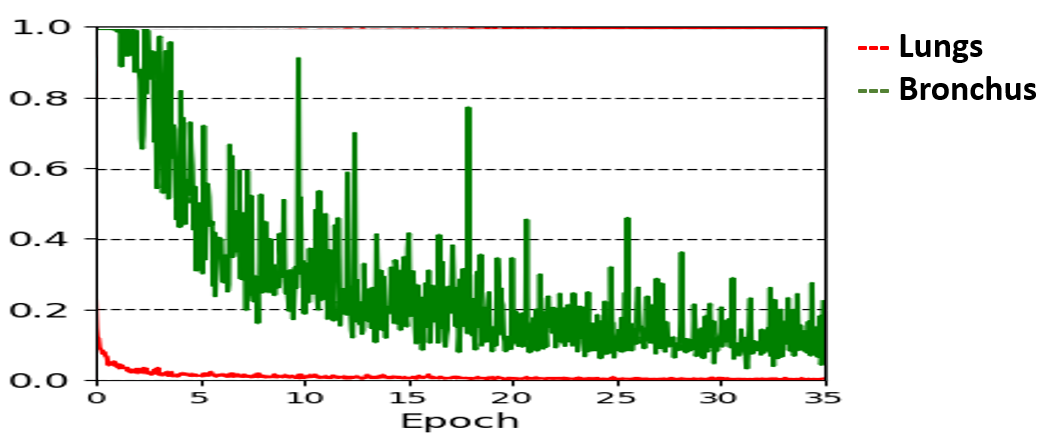
\includegraphics[width=0.49\textwidth, angle=0]{files/deepmedictrain.png}
	\caption{Training process of the DeepMedic architecture. The loss function (BCE) on the training data is shown for the lungs (red) and for the bronchus (green)}
	\label{train_deepmedic}
\end{figure}

The training process for the U-Net architecture is shown in figure \ref{train_unet}. Here the dice loss and the used loss function converge to a asymptote close to 0 on the training set. The metrics on the validation set however do not converge in the same manner. This is caused by overfitting. In some epochs the model creates a too specific representation of the training dataset and is therefore not able to get good results on the validation set. During the training process just models with a improving loss function on the validation set were saved. But in the last 5 epochs the loss function on the validation set decreases to an appropriate value and therefore dthe model is suitable for general predictions. 

\begin{figure}[h!]
	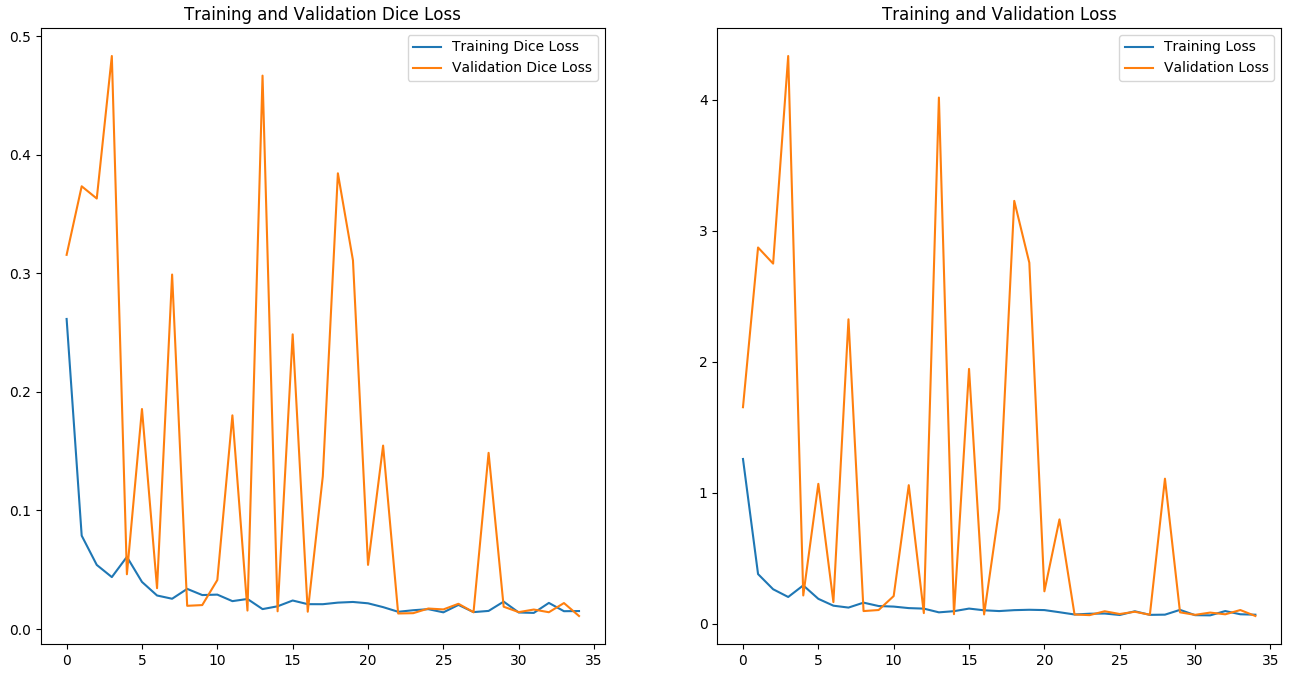
\includegraphics[width=0.49\textwidth, angle=0]{files/jpgunettrain.png}
	\caption{Training process of the U-Net architecture. The dice loss on the training and validation data is shown on the left. The actual loss function ($BCE + dice loss$) is shown on the right.}
	\label{train_unet}
\end{figure}

\subsection{Evaluation of the two architectures}

\begin{figure}[h!]
	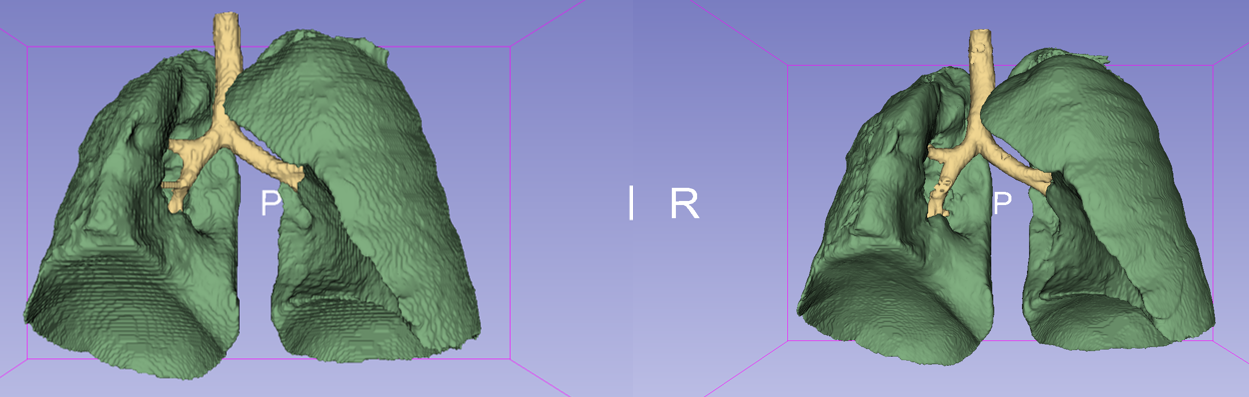
\includegraphics[width=0.49\textwidth, angle=0]{files/preddeepmedic.png}
	\caption{Example prediction of the DeepMedic architecture on one CT scan. The original label map for training is displayed on the left while the prediction of the network is shown on the right.}
	\label{pred_deepmedic}
\end{figure}

For Deepmedic architecture (shown on figure \ref{pred_deepmedic} above), differences between prediction and actual lung are almost indistinguishable at bare eye. Lung's prediction is more smoother than the original. An interesting point is a very precise representation of the bronchus. DeepMedic manages even the small structures thanks to its low-path resolution, seen in chapter \ref{deepmedic_chapter}. This is one point of the divergence to the U-Net results.\newline

\begin{figure}[h!]
	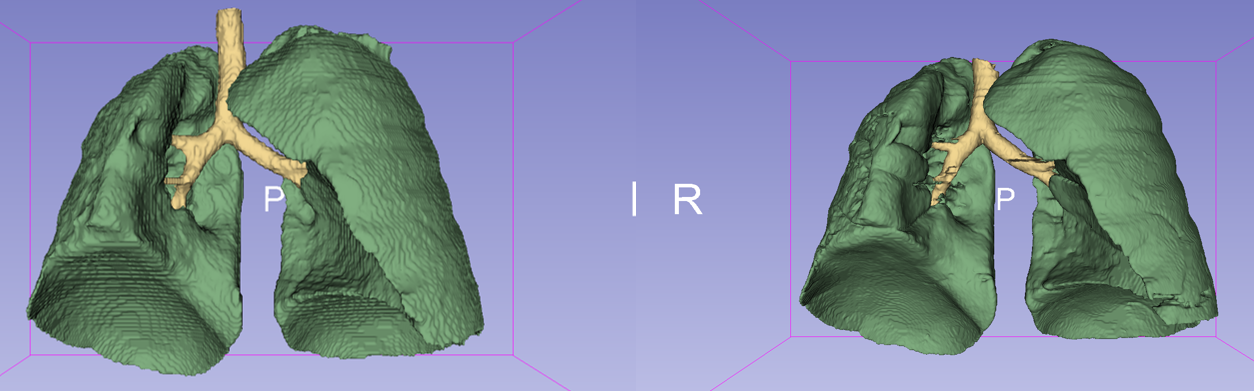
\includegraphics[width=0.49\textwidth, angle=0]{files/predunet.png}
	\caption{Example prediction of the U-Net architecture on one CT scan. The original label map for training is displayed on the left while the prediction of the network is shown on the right.}
	\label{pred_unet}
\end{figure}

Figure \ref{pred_unet} displays an example of the original structure and the predicted scan of the U-Net architecture. The segementation of the bronchus is not as accurate or consistent as it is for Deepmedic. The main reasons for that is that bronchus are more complex, smaller and variable structures. However, the predictions give an appropriate version of the lungs, even slightly better than Deepmedic's ones.\newline\newline

Last part focuses on quantitative analysis over chosen metrics.




comparison of unet and deepmedic

explain high hausdorff and how to reduce it


\begin{table}[h!]
	\caption{Dice Loss, Hausdorff distance and mean distance (on lungs and bronchus) averaged over 20 evaluation CT scans for the DeepMedic and the U-Net architecture.}
	\label{table_result}
	\centering
	\setlength{\tabcolsep}{10pt}
	\renewcommand{\arraystretch}{1.5}
	\begin{tabular}{c c c c}
		\hline 
		Architecture & Dice & Hausdorff & Mean \\
		& Coefficient & distance (mm) & Distance (mm) \\ 
		\hline 
		DeepMedic & 0.968 & 119.50 & 1.45 \\ 
		U-Net & 0.976 & 103.21 & 0.33 \\ 
		\hline
		\newline 
	\end{tabular}

\end{table}
